\section{Curve Sketching}\label{sec:CurveSketching}

In this section, we discuss how we can tell what the graph of a function
looks like by performing simple tests on its derivatives.

%%%%%%%%%%%%%%%%%%%%%%%%%%%%%%%%%%%%%%%%%%%%%%%%%%%%%%%%%%%%
% Subsections to include
%%%%%%%%%%%%%%%%%%%%%%%%%%%%%%%%%%%%%%%%%%%%%%%%%%%%%%%%%%%%
\subsection{Intervals of Increase/Decrease, and the First Derivative Test}\label{sec:FirstDer}
The method of Section~\ref{subsec:LocalExtremaSubsection} for deciding whether there is a
local maximum or minimum at a critical value is not always
convenient. We can instead use information about the derivative
$f'(x)$ to decide; since we have already had to compute the derivative
to find the critical values, there is often relatively little extra
work involved in this method.

How can the derivative tell us whether there is a maximum, minimum, or
neither at a point? Suppose that $f$ is differentiable at and around $x=a$, and suppose further that $a$ is a critical point of $f$. Then we have several possibilities:
\begin{enumerate}
\item	There is a local maximum at $x=a$. This happens if $f'(x)>0$ as we approach $x=a$ from the left (i.e. when $x$ is in the vicinity of $a$, and $x<a$) and $f'(x)<0$ as we move to the right of $x=a$ (i.e. when $x$ is in the vicinity of $a$, and $x>a$).
\item	There is a local minimum at $x=a$. This happens if $f'(x)<0$ as we approach $x=a$ from the left (i.e. when $x$ is in the vicinity of $a$, and $x<a$) and $f'(x)>0$ as we move to the right of $x=a$ (i.e. when $x$ is in the vicinity of $a$, and $x>a$).
\item	There is neither a local maximum or local minimum at $x=a$. If $f'(x)$ does not change from negative to positive, or from positive to negative, as we move from the left of $x=a$ to the right of $x=a$ (that is, $f'(x)$ is positive on both sides of $x=a$, or negative on both sides of $x=a$) then there is neither a maximum nor minimum when $x=a$.
\end{enumerate}
See the first graph in Figure~\ref{fig:max and min points}
and the graph in Figure~\ref{fig:non extremum}
for examples.

\begin{example}{Local Maximum and Minimum}{localmaxandmin}
Find all local maximum and minimum points for $f(x)=\sin x+\cos
x$ using the first derivative test.  
\end{example}

\begin{solution} 
The derivative is $f'(x)=\cos
x-\sin x$ and from Example~\ref{max and min} the critical
values we need to consider are $\pi/4$ and $5\pi/4$.

We analyze the graphs of $\sin x$ and $\cos x$.
Just to the left of $\pi/4$ the cosine is larger than the
  sine, so $f'(x)$ is positive; just to the right the cosine is
  smaller than the sine, so $f'(x)$ is negative. This means there is a
  local maximum at $\pi/4$. Just to the left of $5\pi/4$ the cosine is
  smaller than the sine, and to the right the cosine is larger than
  the sine. This means that the derivative $f'(x)$ is negative to the
  left and positive to the right, so $f$ has a local minimum at
  $5\pi/4$.
\end{solution}

The above observations have obvious intuitive appeal as
you examine the graphs in Figures~\ref{fig:max and min points} and \ref{fig:non extremum}. We can extend these ideas
further and then formulate and prove a theorem: If the graph of $f$ is
increasing before (i.e., to the left of) $x=a$ and decreasing after (i.e.,
to the right of) $x=a,$ then there is a local maximum at $x=a.$ If the graph
of $f$ is decreasing before $x=a$ and increasing after $x=a,$ then there is
a local minimum at $x=a.$ If the graph of $f$ is consistently increasing on
either side of $x=a$ or consistently decreasing on either side of $x=a,$
then there is neither a local maximum nor a local minimum at $x=a.$ We can
prove the following theorem using the Mean Value Theorem.

\begin{theorem}{Intervals of Increase and Decrease}{IntervalsIncDecTheorem}
If $f^{\prime }\left( x\right) >0$ for every $x$ in an interval, then $f$ is
increasing on that interval.

If $f^{\prime }\left( x\right) <0$ for every $x$ in an interval, then $f$ is
decreasing on that interval.
\end{theorem}
\begin{proof}
We will prove the increasing case. The proof of the decreasing case
is similar. Suppose that $f^{\prime }\left( x\right) >0$ on an interval $I.$
Then $f$ is differentiable, and hence also, continuous on $I.$ If $x_{1}$
and $x_{2}$ are any two numbers in $I$ and $x_{1}<x_{2},$ then $f$ is
continuous on $\left[ x_{1},x_{2}\right] $ and differentiable on $\left(
x_{1},x_{2}\right) .$ By the Mean Value Theorem, there is some $c$ in $%
\left( x_{1},x_{2}\right) $ such that 
\begin{equation*}
f^{\prime }\left( c\right) =\frac{f\left( x_{2}\right) -f\left( x_{1}\right) 
}{x_{2}-x_{1}}.
\end{equation*}%
But $c$ must be in $I,$ and thus, since $f^{\prime }\left( x\right) >0$ for
every $x$ in $I,$ $f^{\prime }\left( c\right) >0$. Also, since $x_{1}<x_{2},$
we have $x_{2}-x_{1}>0.$ Therefore, both the left hand side and the
denominator of the right hand side are positive. It follows that the
numerator of the right hand must be positive. That is, $f\left( x_{2}\right)
-f\left( x_{1}\right) >0,$ or in other words, $f\left( x_{1}\right) <f\left(
x_{2}\right) .$ This shows that between $x_{1}$ and $x_{2}$ in $I,$ the
larger one, $x_{2},$ necessarily has the larger function value, $f\left(
x_{2}\right) ,$ and the smaller one, $x_{1},$ necessarily have the smaller
function value, $f\left( x_{1}\right) .$ This means that $f$ is increasing
on $I$.
\end{proof}

\begin{example}{Local Minimum and Maximum}{LocalMaxMinExample}
Consider the function $f\left( x\right) =x^{4}-2x^{2}.$ Find
where $f$ is increasing and where $f$ is decreasing. Use this information to
find the local maximum and minimum points of $f$.
\end{example}
\begin{solution}
We compute $f^{\prime }\left( x\right) $ and analyze its sign. 
\begin{equation*}
f^{\prime }\left( x\right) =4x^{3}-4x=4x\left( x^{2}-1\right) =4x\left(
x-1\right) \left( x+1\right) .
\end{equation*}%
The solution of the inequality $f^{\prime }\left( x\right) >0$ is $\left(
-1,0\right) \cup \left( 1,\infty \right) $. So, $f$ is increasing on the
interval $\left( -1,0\right) $ and on the interval $\left( 1,\infty \right)
. $ The solution of the inequality $f^{\prime }\left( x\right) <0$ is $%
\left( -\infty ,-1\right) \cup \left( 0,1\right) .$ So, $f$ is decreasing on
the interval $\left( -\infty ,-1\right) $ and on the interval $\left(
0,1\right) .$ Therefore, at the critical points $-1,$ $0$ and $1,$
respectively, $f$ has a local minimum, a local maximum and a local minimum.
\end{solution}

%\figure[!ht]
%\vbox{\beginpicture
%\normalgraphs
%%\ninepoint
%\setcoordinatesystem units <1.5truecm,1.5truecm>
%\setplotarea x from 0 to 6.28, y from -1 to 1
%\axis left shiftedto x=0 /
%\axis bottom shiftedto y=0 ticks withvalues {${\pi\over4}$}
%      {$5\pi\over4$} / at 0.7853981635 3.926990818 / /
%\setquadratic
%\plot
%0.000 0.000 
%0.063 0.063 0.126 0.125 0.188 0.187 0.251 0.249 
%0.314 0.309 0.377 0.368 0.440 0.426 0.503 0.482 0.565 0.536 
%0.628 0.588 0.691 0.637 0.754 0.685 0.817 0.729 0.880 0.771 
%0.942 0.809 1.005 0.844 1.068 0.876 1.131 0.905 1.194 0.930 
%1.257 0.951 1.319 0.969 1.382 0.982 1.445 0.992 1.508 0.998 
%1.571 1.000 1.634 0.998 1.696 0.992 1.759 0.982 1.822 0.969 
%1.885 0.951 1.948 0.930 2.011 0.905 2.073 0.876 2.136 0.844 
%2.199 0.809 2.262 0.771 2.325 0.729 2.388 0.685 2.450 0.637 
%2.513 0.588 2.576 0.536 2.639 0.482 2.702 0.426 2.765 0.368 
%2.827 0.309 2.890 0.249 2.953 0.187 3.016 0.125 3.079 0.063 
%3.142 0.000 3.204 -0.063 3.267 -0.125 3.330 -0.187 3.393 -0.249 
%3.456 -0.309 3.519 -0.368 3.581 -0.426 3.644 -0.482 3.707 -0.536 
%3.770 -0.588 3.833 -0.637 3.896 -0.685 3.958 -0.729 4.021 -0.771 
%4.084 -0.809 4.147 -0.844 4.210 -0.876 4.273 -0.905 4.335 -0.930 
%4.398 -0.951 4.461 -0.969 4.524 -0.982 4.587 -0.992 4.650 -0.998 
%4.712 -1.000 4.775 -0.998 4.838 -0.992 4.901 -0.982 4.964 -0.969 
%5.027 -0.951 5.089 -0.930 5.152 -0.905 5.215 -0.876 5.278 -0.844 
%5.341 -0.809 5.404 -0.771 5.466 -0.729 5.529 -0.685 5.592 -0.637 
%5.655 -0.588 5.718 -0.536 5.781 -0.482 5.843 -0.426 5.906 -0.368 
%5.969 -0.309 6.032 -0.249 6.095 -0.187 6.158 -0.125 6.220 -0.063 
%6.283 0.000 /
%\plot
%0.000 1.000 0.063 0.998 0.126 0.992 0.188 0.982 0.251 0.969 
%0.314 0.951 0.377 0.930 0.440 0.905 0.503 0.876 0.565 0.844 
%0.628 0.809 0.691 0.771 0.754 0.729 0.817 0.685 0.880 0.637 
%0.942 0.588 1.005 0.536 1.068 0.482 1.131 0.426 1.194 0.368 
%1.257 0.309 1.319 0.249 1.382 0.187 1.445 0.125 1.508 0.063 
%1.571 0.000 1.634 -0.063 1.696 -0.125 1.759 -0.187 1.822 -0.249 
%1.885 -0.309 1.948 -0.368 2.011 -0.426 2.073 -0.482 2.136 -0.536 
%2.199 -0.588 2.262 -0.637 2.325 -0.685 2.388 -0.729 2.450 -0.771 
%2.513 -0.809 2.576 -0.844 2.639 -0.876 2.702 -0.905 2.765 -0.930 
%2.827 -0.951 2.890 -0.969 2.953 -0.982 3.016 -0.992 3.079 -0.998 
%3.142 -1.000 3.204 -0.998 3.267 -0.992 3.330 -0.982 3.393 -0.969 
%3.456 -0.951 3.519 -0.930 3.581 -0.905 3.644 -0.876 3.707 -0.844 
%3.770 -0.809 3.833 -0.771 3.896 -0.729 3.958 -0.685 4.021 -0.637 
%4.084 -0.588 4.147 -0.536 4.210 -0.482 4.273 -0.426 4.335 -0.368 
%4.398 -0.309 4.461 -0.249 4.524 -0.187 4.587 -0.125 4.650 -0.063 
%4.712 0.000 4.775 0.063 4.838 0.125 4.901 0.187 4.964 0.249 
%5.027 0.309 5.089 0.368 5.152 0.426 5.215 0.482 5.278 0.536 
%5.341 0.588 5.404 0.637 5.466 0.685 5.529 0.729 5.592 0.771 
%5.655 0.809 5.718 0.844 5.781 0.876 5.843 0.905 5.906 0.930 
%5.969 0.951 6.032 0.969 6.095 0.982 6.158 0.992 6.220 0.998 
%6.283 1.000 /
%\endpicture}
%\label{fig:sin and cos}
%\caption{The sine and cosine.}
%\endfigure


%%%%%%%%%%%%%%%%%%%%%%%%%%%%%%%%%%%%%%%%%%%%
\Opensolutionfile{solutions}[ex]
\section*{Exercises for \ref{sec:FirstDer}}

\begin{enumialphparenastyle}

Find all critical points and identify them as local maximum points, local minimum points, or neither.

%%%%%%%%%%
\begin{ex}
 $\ds y=x^2-x$ 
\begin{sol}
 min at $x=1/2$
\end{sol}
\end{ex}

%%%%%%%%%%
\begin{ex}
 $\ds y=2+3x-x^3$ 
\begin{sol}
 min at $x=-1$, max at $x=1$
\end{sol}
\end{ex}

%%%%%%%%%%
\begin{ex}
 $\ds y=x^3-9x^2+24x$
\begin{sol}
 max at $x=2$, min at $x=4$
\end{sol}
\end{ex}

%%%%%%%%%%
\begin{ex}
 $\ds y=x^4-2x^2+3$ 
\begin{sol}
 min at $x=\pm 1$, max at $x=0$.
\end{sol}
\end{ex}

%%%%%%%%%%
\begin{ex}
 $\ds y=3x^4-4x^3$
\begin{sol}
 min at $x=1$
\end{sol}
\end{ex}

%%%%%%%%%%
\begin{ex}
 $\ds y=(x^2-1)/x$
\begin{sol}
 none
\end{sol}
\end{ex}

%%%%%%%%%%
\begin{ex}
 $\ds y=3x^2-(1/x^2)$ 
\begin{sol}
 none
\end{sol}
\end{ex}

%%%%%%%%%%
\begin{ex}
 $y=\cos(2x)-x$ 
\begin{sol}
 min at $x=7\pi/12+k\pi$, max at $x=-\pi/12+k\pi$, for integer $k$.
\end{sol}
\end{ex}

%%%%%%%%%%
\begin{ex}
$\ds f(x) = (5-x)/(x+2)$
\begin{sol}
 none
\end{sol}
\end{ex}

%%%%%%%%%%
\begin{ex}
 $\ds f(x) = |x^2 - 121|$
\begin{sol}
 max at $x=0$, min at $x=\pm 11$
\end{sol}
\end{ex}

%%%%%%%%%%
\begin{ex}
 $\ds f(x) = x^3/(x+1)$
\begin{sol}
 min at $x=-3/2$, neither at $x=0$
\end{sol}
\end{ex}

%%%%%%%%%%%
%\begin{ex}
% $\ds f(x)= \cases{x^2 \sin(1/x)  & $x\neq 0$ \cr
% 0  & $x=0$\cr}$

%%%%%%%%%%
\begin{ex}
 $\ds f(x) = \sin ^2 x$
\begin{sol}
 min at $n\pi$, max at $\pi/2+n\pi$
\end{sol}
\end{ex}

%%%%%%%%%%
\begin{ex}
 Find the maxima and minima of $f(x)=\sec x$.
\begin{sol}
 min at $2n\pi$, max at $(2n+1)\pi$
\end{sol}
\end{ex}

%%%%%%%%%%
\begin{ex}
  Let $\ds f(\theta) = \cos^2(\theta) -
 2\sin(\theta)$.  Find the intervals where $f$ is increasing and the
 intervals where $f$ is decreasing in $[0,2\pi]$.  Use this
 information to classify the critical points of $f$ as either local
 maximums, local minimums, or neither.
\begin{sol}
 min at $\pi/2+2n\pi$, max at $3\pi/2+2n\pi$
\end{sol}
\end{ex}

%%%%%%%%%%
\begin{ex}
 Let $r>0$. Find the local
maxima and minima of the function $\ds f(x)
=\sqrt{r^2 -x^2 }$ on its domain $[-r,r]$.
\end{ex}

%%%%%%%%%%
\begin{ex}
 Let $\ds f(x) =a x^2 + bx + c$ with $a\neq 0$. Show that $f$
has exactly one critical point using the first derivative test. Give
conditions on $a$ and $b$ which guarantee that the critical point will
be a maximum. It is possible to see this without using calculus at
all; explain.
\end{ex}

\end{enumialphparenastyle}
\subsection{The Second Derivative Test}\label{sec:SecondDer}
The basis of the first derivative test is that if the derivative
changes from positive to negative at a point at which the derivative
is zero then there is a local maximum at the point, and similarly for
a local minimum. If $f'$ changes from positive to negative it is
decreasing; this means that the derivative of $f'$, $f''$, might be negative,
and if in fact $f''$ is negative then $f'$ is definitely
decreasing. From this we determine that there is a local maximum at the point in question. Note
that $f'$ might change from positive to negative while $f''$ is
zero, in which case $f''$ gives us no information about the critical
value. Similarly, if $f'$ changes from negative to positive there is a
local minimum at the point, and $f'$ is increasing. If $f''>0$ at the
point, this tells us that $f'$ is increasing, and so there is a local
minimum.

\begin{example}{Second Derivative}{secondderivative}
Consider again $f(x)=\sin x + \cos x$,  with $f'(x)=\cos x-\sin x$ and
$ f''(x)=-\sin x -\cos x$. Use the second derivative test to determine which critical points are local maximum or minima.
\end{example}
\begin{solution}
Since $\ds f''(\pi/4)=-\sqrt{2}/2-\sqrt2/2=-\sqrt2<0$,
we know there is a local maximum at $\pi/4$. Since
$\ds f''(5\pi/4)=-(-\sqrt{2}/2)-(-\sqrt2/2)=\sqrt2>0$, there is a local
minimum at $5\pi/4$.
\end{solution}

When it works, the second derivative test is often the easiest way to
identify local maximum and minimum points. Sometimes the test fails,
and sometimes the second derivative is quite difficult to evaluate; in
such cases we must fall back on one of the previous tests.

\begin{example}{Second Derivative}{secondderivativetwo}
Let $\ds f(x)=x^4$ and $\ds g(x)=-x^4$. Classify the critical points of $f(x)$ and $g(x)$ as either maximum or minimum.
\end{example}
\begin{solution}
The derivatives for $f(x)$ are $f'(x)=4x^3$ and $\ds f''(x)=12x^2$.
Zero is the only critical value, but $f''(0)=0$, so
the second derivative test tells us nothing. However, $f(x)$ is
positive everywhere except at zero, so clearly $f(x)$ has a local
minimum at zero.

On the other hand, for $g(x)=-x^4$, $g'(x)=-4x^3$ and $g''(x)=-12x^2$. So $g(x)$ also has zero
as its only only critical value, and the second derivative is again zero, but $-x^4$ has a local maximum at zero.
\end{solution}


%%%%%%%%%%%%%%%%%%%%%%%%%%%%%%%%%%%%%%%%%%%%
\Opensolutionfile{solutions}[ex]
\section*{Exercises for \ref{sec:SecondDer}}

\begin{enumialphparenastyle}

Find all local maximum and minimum points by the second derivative test. 


%%%%%%%%%%
\begin{ex}
 $\ds y=x^2-x$ 
\begin{sol}
 min at $x=1/2$
\end{sol}
\end{ex}

%%%%%%%%%%
\begin{ex}
 $\ds y=2+3x-x^3$ 
\begin{sol}
 min at $x=-1$, max at $x=1$
\end{sol}
\end{ex}

%%%%%%%%%%
\begin{ex}
 $\ds y=x^3-9x^2+24x$
\begin{sol}
 max at $x=2$, min at $x=4$
\end{sol}
\end{ex}

%%%%%%%%%%
\begin{ex}
 $\ds y=x^4-2x^2+3$ 
\begin{sol}
 min at $x=\pm 1$, max at $x=0$.
\end{sol}
\end{ex}

%%%%%%%%%%
\begin{ex}
 $\ds y=3x^4-4x^3$
\begin{sol}
 min at $x=1$
\end{sol}
\end{ex}

%%%%%%%%%%
\begin{ex}
 $\ds y=(x^2-1)/x$
\begin{sol}
 none
\end{sol}
\end{ex}

%%%%%%%%%%
\begin{ex}
 $\ds y=3x^2-(1/x^2)$ 
\begin{sol}
 none
\end{sol}
\end{ex}

%%%%%%%%%%
\begin{ex}
 $y=\cos(2x)-x$ 
\begin{sol}
 min at $x=7\pi/12+n\pi$, max at $x=-\pi/12+n\pi$, for integer $n$.
\end{sol}
\end{ex}

%%%%%%%%%%
\begin{ex}
 $\ds y = 4x+\sqrt{1-x}$
\begin{sol}
 max at $x=63/64$
\end{sol}
\end{ex}

%%%%%%%%%%
\begin{ex}
 $\ds y = (x+1)/\sqrt{5x^2 + 35}$
\begin{sol}
 max at $x=7$
\end{sol}
\end{ex}

%%%%%%%%%%
\begin{ex}
 $\ds y= x^5 - x$
\begin{sol}
 max at $\ds -5^{-1/4}$, min at $\ds 5^{-1/4}$
\end{sol}
\end{ex}

%%%%%%%%%%
\begin{ex}
 $\ds y = 6x +\sin 3x$
\begin{sol}
 none
\end{sol}
\end{ex}

%%%%%%%%%%
\begin{ex}
 $\ds y = x+ 1/x$
\begin{sol}
 max at $-1$, min at $1$
\end{sol}
\end{ex}

%%%%%%%%%%
\begin{ex}
 $\ds y = x^2+ 1/x$
\begin{sol}
 min at $\ds 2^{-1/3}$
\end{sol}
\end{ex}

%%%%%%%%%%
\begin{ex}
 $\ds y = (x+5)^{1/4}$
\begin{sol}
 none
\end{sol}
\end{ex}

%%%%%%%%%%
\begin{ex}
 $\ds y = \tan^2 x$
\begin{sol}
 min at $n\pi$
\end{sol}
\end{ex}

%%%%%%%%%%
\begin{ex}
 $\ds y =\cos^2 x - \sin^2 x$
\begin{sol}
 max at $n\pi$, min at $\pi/2+n\pi$
\end{sol}
\end{ex}

%%%%%%%%%%
\begin{ex}
 $\ds y = \sin^3 x$
\begin{sol}
 max at $\pi/2+2n\pi$, min at $3\pi/2+2n\pi$
\end{sol}
\end{ex}

\end{enumialphparenastyle}
\subsection{Concavity and Inflection Points}\label{sec:Concavity}
We know that the sign of the derivative tells us whether a function is
increasing or decreasing; for example, when $f'(x)>0$,
$f(x)$ is increasing. The sign of the second derivative
$f''(x)$ tells us whether $f'$ is increasing or decreasing; we have
seen that if $f'$ is zero and increasing at a point then there is a
local minimum at the point. If $f'$ is zero and decreasing at a
point then there is a local maximum at the point. Thus, we extracted
information about $f$ from information about $f''$. 

We can get information from the sign of $f''$ even when $f'$ is not
zero. Suppose that $f''(a)>0$. This means that near $x=a$, $f'$ is
increasing. If $f'(a)>0$, this means that $f$ slopes up and is getting
steeper; if $f'(a)<0$, this means that $f$ slopes down and is getting
{\it less} steep. The two situations are shown in
figure~\ref{fig:concave up}. A curve that is shaped like this is
called \dfont{concave up}.


\figure[H]
\centerline{\vbox{\beginpicture
\normalgraphs
%\ninepoint
\setcoordinatesystem units <2truecm,2truecm>
\setplotarea x from 0 to 1, y from 0 to 1
\axis left shiftedto x=0 /
\axis bottom shiftedto y=0 ticks withvalues {$a$} / at 0.5 / /
\setquadratic
\plot 0.1 0.2 0.5 0.4 0.9 0.9 /
\setcoordinatesystem units <2truecm,2truecm> point at -2 0
\setplotarea x from 0 to 1, y from 0 to 1
\axis left shiftedto x=0 /
\axis bottom shiftedto y=0 ticks withvalues {$a$} / at 0.5 / /
\setquadratic
\plot 0.1 0.9 0.5 0.3 0.9 0.1 /
\endpicture}}
\caption{$f''(a)>0$: $f'(a)$ positive and increasing, $f'(a)$ negative and
  increasing. \label{fig:concave up}}
\endfigure

Now suppose that $f''(a)<0$. This means that near $x=a$, $f'$ is
decreasing. If $f'(a)>0$, this means that $f$ slopes up and is getting
less steep; if $f'(a)<0$, this means that $f$ slopes down and is getting
steeper. The two situations are shown in
figure~\ref{fig:concave down}. A curve that is shaped like this is
called \dfont{concave down}.


\figure[H]
\centerline{\vbox{\beginpicture
\normalgraphs
%\ninepoint
\setcoordinatesystem units <2truecm,2truecm>
\setplotarea x from 0 to 1, y from 0 to 1
\axis left shiftedto x=0 /
\axis bottom shiftedto y=0 ticks withvalues {$a$} / at 0.5 / /
\setquadratic
\plot 0.1 0.2 0.5 0.7 0.9 0.9 /
\setcoordinatesystem units <2truecm,2truecm> point at -2 0
\setplotarea x from 0 to 1, y from 0 to 1
\axis left shiftedto x=0 /
\axis bottom shiftedto y=0 ticks withvalues {$a$} / at 0.5 / /
\setquadratic
\plot 0.1 0.9 0.5 0.6 0.9 0.1 /
\endpicture}}
\caption{$f''(a)<0$: $f'(a)$ positive and decreasing, $f'(a)$ negative and
  decreasing. \label{fig:concave down}}
\endfigure

If we are trying to understand the shape of the graph of a function,
knowing where it is concave up and concave down helps us to get a more
accurate picture. Of particular interest are points at which the
concavity changes from up to down or down to up; such points are
called \dfont{inflection points}. If the
concavity changes from up to down at $x=a$, $f''$ changes from
positive to the left of $a$ to negative to the right of $a$, and
usually $f''(a)=0$. We can identify such points by first finding where
$f''(x)$ is zero and then checking to see whether $f''(x)$ does in
fact go from positive to negative or negative to positive at these
points. Note that it is possible that $f''(a)=0$ but the concavity is
the same on both sides; $\ds f(x)=x^4$ at $x=0$ is an example.

\begin{example}{Concavity}{concavity}
Describe the concavity of $\ds f(x)=x^3-x$.
\end{example}
\begin{solution}
The derivatives are $\ds f'(x)=3x^2-1$ and $f''(x)=6x$.
Since $f''(0)=0$, there is potentially an inflection point at
zero. Since $f''(x)>0$ when $x>0$ and $f''(x)<0$ when $x<0$ the
concavity does change from concave down to concave up at zero, and the curve is
concave down for all $x<0$ and concave up for all $x>0$.
\end{solution}

Note that we need to compute and analyze the second derivative to
understand concavity, so we may as well try to use the second
derivative test for maxima and minima. If for some reason this fails
we can then try one of the other tests.


%%%%%%%%%%%%%%%%%%%%%%%%%%%%%%%%%%%%%%%%%%%%
\Opensolutionfile{solutions}[ex]
\section*{Exercises for \ref{sec:Concavity}}

\begin{enumialphparenastyle}

Describe the concavity of the functions below.

%%%%%%%%%%
\begin{ex}
 $\ds y=x^2-x$ 
\begin{sol}
 concave up everywhere
\end{sol}
\end{ex}

%%%%%%%%%%
\begin{ex}
 $\ds y=2+3x-x^3$ 
\begin{sol}
 concave up when $x<0$, concave down when $x>0$
\end{sol}
\end{ex}

%%%%%%%%%%
\begin{ex}
 $\ds y=x^3-9x^2+24x$
\begin{sol}
 concave down when $x<3$, concave up when $x>3$
\end{sol}
\end{ex}

%%%%%%%%%%
\begin{ex}
 $\ds y=x^4-2x^2+3$ 
\begin{sol}
 concave up when $\ds x<-1/\sqrt3$ or $\ds x>1/\sqrt3$,
concave down when $\ds -1/\sqrt3<x<1/\sqrt3$
\end{sol}
\end{ex}

%%%%%%%%%%
\begin{ex}
 $\ds y=3x^4-4x^3$
\begin{sol}
 concave up when $x<0$ or $x>2/3$,
concave down when $0<x<2/3$
\end{sol}
\end{ex}

%%%%%%%%%%
\begin{ex}
 $\ds y=(x^2-1)/x$
\begin{sol}
 concave up when $x<0$, concave down when $x>0$
\end{sol}
\end{ex}

%%%%%%%%%%
\begin{ex}
 $\ds y=3x^2-(1/x^2)$ 
\begin{sol}
 concave up when $x<-1$ or $x>1$, concave down when
$-1<x<0$ or $0<x<1$
\end{sol}
\end{ex}

%%%%%%%%%%
\begin{ex}
 $y=\sin x + \cos x$ 
\begin{sol}
 concave down on $((8n-1)\pi/4,(8n+3)\pi/4)$,
concave up on $((8n+3)\pi/4,(8n+7)\pi/4)$, for integer $n$
\end{sol}
\end{ex}

%%%%%%%%%%
\begin{ex}
 $\ds y = 4x+\sqrt{1-x}$
\begin{sol}
 concave down everywhere
\end{sol}
\end{ex}

%%%%%%%%%%
\begin{ex}
 $\ds y = (x+1)/\sqrt{5x^2 + 35}$
\begin{sol}
 concave up on $\ds (-\infty,(21-\sqrt{497})/4)$ and 
$\ds (21+\sqrt{497})/4,\infty)$
\end{sol}
\end{ex}

%%%%%%%%%%
\begin{ex}
 $\ds y= x^5 - x$
\begin{sol}
 concave up on $(0,\infty)$
\end{sol}
\end{ex}

%%%%%%%%%%
\begin{ex}
 $\ds y = 6x + \sin 3x$
\begin{sol}
 concave down on $(2n\pi/3,(2n+1)\pi/3)$
\end{sol}
\end{ex}

%%%%%%%%%%
\begin{ex}
 $\ds y = x+ 1/x$
\begin{sol}
 concave up on $(0,\infty)$
\end{sol}
\end{ex}

%%%%%%%%%%
\begin{ex}
 $\ds y = x^2+ 1/x$
\begin{sol}
 concave up on $(-\infty,-1)$ and $(0,\infty)$
\end{sol}
\end{ex}

%%%%%%%%%%
\begin{ex}
 $\ds y = (x+5)^{1/4}$
\begin{sol}
 concave down everywhere
\end{sol}
\end{ex}

%%%%%%%%%%
\begin{ex}
 $\ds y = \tan^2 x$
\begin{sol}
 concave up everywhere
\end{sol}
\end{ex}

%%%%%%%%%%
\begin{ex}
 $\ds y =\cos^2 x - \sin^2 x$
\begin{sol}
 concave up on $(\pi/4+n\pi,3\pi/4+n\pi)$
\end{sol}
\end{ex}

%%%%%%%%%%
\begin{ex}
 $\ds y = \sin^3 x$
\begin{sol}
 inflection points at $n\pi$, $\ds \pm\arcsin(\sqrt{2/3})+n\pi$
\end{sol}
\end{ex}

%%%%%%%%%%
\begin{ex}
 Identify the intervals on which the graph of the function
$\ds f(x) = x^4-4x^3 +10$ is of one of these four
shapes: concave up and increasing; concave up and decreasing; concave
down and increasing; concave down and decreasing.
\begin{sol}
 up/incr: $(3,\infty)$, up/decr: $(-\infty,0)$, $(2,3)$,
down/decr: $(0,2)$
\end{sol}
\end{ex}

%%%%%%%%%%
\begin{ex}
 Describe the concavity of $\ds y =  x^3 + bx^2 + cx + d$.
You will need to consider different cases, depending on the values of
the coefficients.
\end{ex}

%%%%%%%%%%
\begin{ex}
 Let $n$ be an integer greater than or equal to
two, and suppose $f$ is a polynomial of degree $n$. How many inflection points
can $f$ have?  Hint: Use the second derivative test and the
fundamental theorem of algebra.
\end{ex}

\end{enumialphparenastyle}
\subsection{Asymptotes and Other Things to Look For}\label{sec:Asymptotes}
A vertical asymptote\index{asymptote} is a place where the function
becomes infinite, typically because the formula for the function has a
denominator that becomes zero.  For example, the reciprocal function
$f(x)=1/x$ has a vertical asymptote at $x=0$, and the function $\tan
x$ has a vertical asymptote at $x=\pi/2$ (and also at $x=-\pi/2$,
$x=3\pi/2$, etc.).  Whenever the formula for a function contains a
denominator it is worth looking for a vertical asymptote by 
checking to see if the denominator can ever be zero, and then checking
the limit at such points. Note that there is not always a vertical
asymptote where the derivative is zero: $f(x)=(\sin x)/x$ has a zero
denominator at $x=0$, but since $\ds \lim_{x\to 0}(\sin x)/x=1$ there is
no asymptote there.

A horizontal asymptote is a horizontal line to which $f(x)$ gets closer and
closer as $x$ approaches $\infty$ (or as $x$ approaches $-\infty$).  For
example, the reciprocal function has the $x$-axis for a horizontal
asymptote.  Horizontal asymptotes can be identified by computing 
the limits $\ds \lim_{x \to \infty}f(x)$ and $\ds \lim_{x \to -\infty}f(x)$.
Since $\ds \lim_{x \to \infty}1/x=\lim_{x \to -\infty}1/x=0$, the line
$y=0$ (that is, the $x$-axis) is a horizontal asymptote in both directions.

Some functions have asymptotes that are neither horizontal nor
vertical, but some other line. Such asymptotes are somewhat more
difficult to identify and we will ignore them.

If the domain of the function does not extend out to infinity, we should
also ask what happens as $x$ approaches the boundary of the domain.  For
example, the function $\ds y=f(x)=1/\sqrt{r^2-x^2}$ has domain $-r<x<r$, and
$y$ becomes infinite as $x$ approaches either $r$ or $-r$. In this
case we might also identify this behavior because when $x=\pm r$ the
denominator of the function is zero.

If there are any points where the derivative fails to exist (a cusp or
corner), then we should take special note of what the function does at such
a point.

Finally, it is worthwhile to notice any symmetry.  A function $f(x)$ that
has the same value for $-x$ as for $x$, i.e., $f(-x)=f(x)$, is called an
``even function.''  Its graph is symmetric with respect to the $y$-axis.
Some examples of even functions are: $\ds x^n$ when $n$ is an even number,
$\cos x$, and $\ds \sin^2x$.  On the other hand, a function that satisfies the
property $f(-x)=-f(x)$ is called an ``odd function.''  Its graph is
symmetric with respect to the origin.  Some examples of odd functions are:
$x^n$ when $n$ is an odd number, $\sin x$, and $\tan x$.  Of course, most
functions are neither even nor odd, and do not have any particular
symmetry.
\subsection{Summary of Curve Sketching}\label{subsec:SummaryCurveSketching}

The following is a guideline for sketching a curve $y=f(x)$ by hand. Each item may not be relevant to the function in question, but utilizing this guideline will provide all information needed to make a detailed sketch of the function.

\begin{formulabox}[Guideline for Curve Sketching]
\begin{enumerate}
	\item	Domain of the function
	\item	$x$- and $y$-Intercepts
	\item	Symmetry
	\item	Vertical and Horizontal Asymptotes
	\item	Intervals of Increase/Decrease, and Local Extrema
	\item	Concavity and Points of Inflection
	\item	Sketch the Graph
\end{enumerate}
\end{formulabox}

\begin{example}{Graph Sketching}{graphsketching}
Sketch the graph of $y=f(x)$ where $\ds{f(x)=\frac{2x^2}{x^2-1}}$
\end{example}

\begin{solution} 
\begin{enumerate}
\item  The domain is $\{x: x^2-1 \neq 0\}= \{x: x \neq \pm 1\}=(- \infty,-1) \cup (-1,1) \cup (1, \infty)$
\item  There is an $x$-intercept at $x=0$. The $y$ intercept is $y=0$.
\item  $f(-x)=f(x)$, so $f$ is an even function (symmetric about $y$-axis)
\item  $\ds{ \lim_{x \to \pm \infty} \frac{2x^2}{x^2-1} =\lim_{x \to \pm \infty} \frac{2}{1-1/x^2} = 2 }$, so $y=2$ is a horizontal asymptote.

Now the denominator is 0 at $x =\pm1$, so we compute:
\[\lim_{x \to 1^+} \frac{2x^2}{x^2-1} = + \infty, \;   \lim_{x \to 1^-} \frac{2x^2}{x^2-1} = - \infty, \;
\lim_{x \to -1^+} \frac{2x^2}{x^2-1} = - \infty, \;   \lim_{x \to -1^-} \frac{2x^2}{x^2-1} = + \infty.  \]
So the lines $x=1$ and $x=-1$ are vertical asymptotes. 

\item  For critical values we take the derivative:
$$f'(x) = \frac{4x(x^2-1)-2x^2 \cdot 2x}{(x^2-1)^2} = \frac{-4x}{(x^2-1)^2}.$$
Note that $f'(x)=0$ when $x=0$ (the top is zero).
Also, $f'(x)=DNE$ when $x=\pm 1$ (the bottom is zero).
As $x=\pm 1$ is \ifont{not} in the domain of $f(x)$, the only critical number is $x=0$ (recall that to be a critical number we need it to be in the domain of the original function).

Drawing a number line and including \ifont{all} of the split points of $f'(x)$ we have:
$$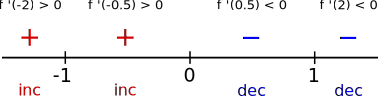
\includegraphics[width=3.5in]{images/graphex1}$$
Thus $f$ is increasing on $(-\infty, -1)\cup(-1,0)$ and decreasing on $(0,1)\cup(1, \infty)$.

By the first derivative test, $x=0$ is a local max.

\item  For possible inflection points we take the second derivative:
$$f''(x)= \frac{12x^2+4}{(x^2-1)^3}$$
The top is never zero.
Also, the bottom is only zero when $x=\pm 1$ (neither of which are in the domain of $f(x)$).
Thus, there are no possible inflection points to consider.

Drawing a number line and including \ifont{all} of the split points of $f''(x)$ we have:
$$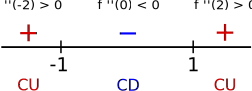
\includegraphics[width=2.25in]{images/graphex2}$$
Hence $f$ is concave up on $(- \infty,-1)\cup(1, \infty)$, concave down on $(-1,1)$.

\item  We put this information together and sketch the graph.

We combine some of this information on a single number line to see what \ifont{shape} the graph has on certain intervals:
$$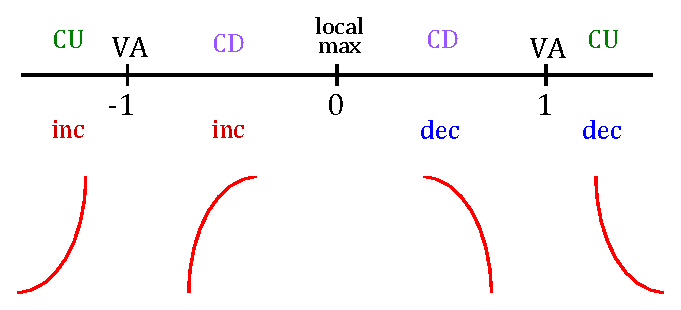
\includegraphics[width=3.0in]{images/graphex3}$$
Note that there is a horizontal asymptote at $y=2$ and that the curve has $x$-int of $x=0$ and $y$-int of $y=0$.
Therefore, a sketch of $f(x)$ is as follows:
$$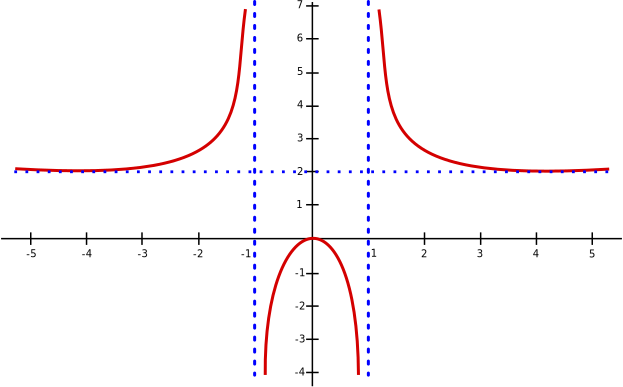
\includegraphics[width=3.5in]{images/graphex4}$$
\end{enumerate}
\end{solution}

% Exercises are included at the end of each subsection, except the 'asymptotes-other' subsection which does not have its own exercises
% The following are exercises for the entire section on Curve Sketching


%%%%%%%%%%%%%%%%%%%%%%%%%%%%%%%%%%%%%%%%%%%%
\Opensolutionfile{solutions}[ex]
\section*{Exercises for \ref{sec:CurveSketching}}

\begin{enumialphparenastyle}

Sketch the curves. Identify clearly any interesting features, including
local maximum and minimum points, inflection points, asymptotes, and
intercepts. 

%%%%%%%%%%
\begin{ex}
	$\ds y=x^5-5x^4+5x^3$
\end{ex}

%%%%%%%%%%
\begin{ex}
	$\ds y=x^3-3x^2-9x+5$
\end{ex}

%%%%%%%%%%
\begin{ex}
	$\ds y=(x-1)^2(x+3)^{2/3}$
\end{ex}

%%%%%%%%%%
\begin{ex}
	$\ds x^2+x^2y^2=a^2y^2$, $a>0$.
\end{ex}

%%%%%%%%%%
\begin{ex}
	$\ds y=xe^x$
\end{ex}

%%%%%%%%%%
\begin{ex}
	$\ds y=(e^x+e^{-x})/2$
\end{ex}

%%%%%%%%%%
\begin{ex}
	$\ds y=e^{-x}\cos x$
\end{ex}

%%%%%%%%%%
\begin{ex}
	$\ds y=e^x-\sin x$
\end{ex}

%%%%%%%%%%
\begin{ex}
	$\ds y=e^x/x$
\end{ex}

%%%%%%%%%%
\begin{ex}
	$\ds y = 4x+\sqrt{1-x}$
\end{ex}

%%%%%%%%%%
\begin{ex}
	$\ds y = (x+1)/\sqrt{5x^2 + 35}$
\end{ex}

%%%%%%%%%%
\begin{ex}
	$\ds y= x^5 - x$
\end{ex}

%%%%%%%%%%
\begin{ex}
	$\ds y = 6x + \sin 3x$
\end{ex}

%%%%%%%%%%
\begin{ex}
	$\ds y = x+ 1/x$
\end{ex}

%%%%%%%%%%
\begin{ex}
	$\ds y = x^2+ 1/x$
\end{ex}

%%%%%%%%%%
\begin{ex}
	$\ds y = (x+5)^{1/4}$
\end{ex}

%%%%%%%%%%
\begin{ex}
	$\ds y = \tan^2 x$
\end{ex}

%%%%%%%%%%
\begin{ex}
	$\ds y =\cos^2 x - \sin^2 x$
\end{ex}

%%%%%%%%%%
\begin{ex}
	$\ds y = \sin^3 x$
\end{ex}

%%%%%%%%%%
\begin{ex}
	$\ds y=x(x^2+1)$
\end{ex}

%%%%%%%%%%
\begin{ex}
	$\ds y=x^3+6x^2 + 9x$
\end{ex}

%%%%%%%%%%
\begin{ex}
	$\ds y=x/(x^2-9)$
\end{ex}

%%%%%%%%%%
\begin{ex}
	$\ds y=x^2/(x^2+9)$
\end{ex}

%%%%%%%%%%
\begin{ex}
	$\ds y=2\sqrt{x} - x$
\end{ex}

%%%%%%%%%%
\begin{ex}
	$\ds y=3\sin(x) - \sin^3(x)$, for $x\in[0,2\pi]$
\end{ex}

%%%%%%%%%%
\begin{ex}
	$\ds y=(x-1)/(x^2)$
\end{ex}

\end{enumialphparenastyle}